\begin{center}
	\chapter{RESULTS AND ANALYSIS}
\end{center}
\justifying

\section{Baseline Reproduction}

The base architecture was rebuilt from the reference implementation and its
published state-tracking behaviour reproduced on the available hardware. On
$S_3$, the published contrast is recovered exactly: $n_h = 2$ reaches sequence
accuracy $1.000$ within a single epoch, while $n_h = 1$ remains at $0.000$,
consistent with the requirement of two factors for a three-cycle. On $S_5$ with
$n_h = 4$, trained on $500{,}000$ sequences for $100$ epochs, the model attains
token accuracy $0.864$ at sequence length $512$ after training at length $128$,
with whole-sequence accuracy perfect through position $121$. The length
extrapolation behaviour matches the published result qualitatively.

This baseline underlies every comparison reported below.

\section{Reachability of Permutation Transitions}

Every element of $S_5$ was reconstructed by explicit construction at every factor
count $K$ from zero to four, under a free $\beta$ and under $\beta$ held at $2$.
All $120$ elements were treated at each $K$, and the worst reconstruction error
over the entire set was $1.17 \times 10^{-15}$. Table \ref{table:reach} records
which combinations admit an exact representation.

\begin{table}[ht]
	\caption{Reachability of permutations of transposition length $\ell$ using $K$ factors. A tick denotes exact representation; a dash denotes that no exact representation exists.}
	\centering
	\begin{tabular}{c c c c c c | c c c c c}
		\hline\hline
		& \multicolumn{5}{c|}{Learnable $\beta \in [0,2]$} & \multicolumn{5}{c}{Fixed $\beta = 2$} \\
		$\ell$ & $K{=}0$ & $K{=}1$ & $K{=}2$ & $K{=}3$ & $K{=}4$ & $K{=}0$ & $K{=}1$ & $K{=}2$ & $K{=}3$ & $K{=}4$ \\ [0.5ex]
		\hline
		0 & \checkmark & \checkmark & \checkmark & \checkmark & \checkmark & \checkmark & --         & \checkmark & --         & \checkmark \\
		1 & --         & \checkmark & \checkmark & \checkmark & \checkmark & --         & \checkmark & --         & \checkmark & --         \\
		2 & --         & --         & \checkmark & \checkmark & \checkmark & --         & --         & \checkmark & --         & \checkmark \\
		3 & --         & --         & --         & \checkmark & \checkmark & --         & --         & --         & \checkmark & --         \\
		4 & --         & --         & --         & --         & \checkmark & --         & --         & --         & --         & \checkmark \\ [1ex]
		\hline
	\end{tabular}
	\label{table:reach}
\end{table}

The left half exhibits the rank bound alone: every $K \ge \ell$ is reachable. The
right half exhibits both bounds acting together, and the alternating pattern is
the determinant-parity constraint, under which exactly half of the admissible
combinations are lost. This result is what fixes the placement of the gate on the
factor strength rather than on a selection between fixed values, as described in
Section \ref{sec:mechanism}.

\section{Verification of the Order-Requirement Model}

The three-dimensional faithful representation of $A_5$ was constructed
independently from geometry, as the rotation group of the icosahedron, and
verified against the properties the model requires. The construction yields $60$
distinct rotations closed under composition with a closure error of
$1.4 \times 10^{-16}$; the element-order profile is
$\{1{:}1,\ 2{:}15,\ 3{:}20,\ 5{:}24\}$, which is that of $A_5$; and the
isomorphism is exhibited explicitly through the action on the five inscribed
octahedra, verified to be faithful, to have even image, and to be surjective onto
all $60$ elements. Every non-identity element of the representation has
$\operatorname{rank}(\rho(g) - I) = 2$, and each factors into exactly two
Householder reflections with a worst reconstruction error of
$1.31 \times 10^{-15}$.

Table \ref{table:a5} sets the resulting requirement against the transposition
length for each conjugacy class. The two quantities agree except on the
five-cycles, where they differ by a factor of two.

\begin{table}[ht]
	\caption{Transposition length and order requirement within $A_5$}
	\centering
	\begin{tabular}{P{4.2cm} c c c}
		\hline\hline
		Element type & Count & $\ell$ (permutation rep.) & $D$ (3-D rep.) \\ [0.5ex]
		\hline
		Identity & 1 & 0 & 0 \\
		Double transposition & 15 & 2 & 2 \\
		Three-cycle & 20 & 2 & 2 \\
		Five-cycle & 24 & 4 & 2 \\ [1ex]
		\hline
	\end{tabular}
	\label{table:a5}
\end{table}

\section{Alphabet Closure as a Predictor of Trainability}

Section \ref{sec:demand} predicts that the generated group, rather than the
alphabet size or the identity of the individual symbols, determines the required
factor count. The prediction was tested by holding the factor count at
$n_h = 3$, one below the requirement of $S_5$ and one above the requirement of
$A_5$, and varying the alphabet across the closure boundary. Under the
order-requirement model, alphabets generating $A_5$ should be solvable at this
factor count and alphabets generating $S_5$ should not, irrespective of their
size. Table \ref{table:closure} reports the outcome.

\begin{table}[ht]
	\caption{Trainability at $n_h = 3$ as a function of the group generated by the alphabet}
	\centering
	\begin{tabular}{P{6.0cm} c c}
		\hline\hline
		Alphabet & Generated group & Token accuracy \\ [0.5ex]
		\hline
		24 five-cycles & $A_5$ & 0.9991 \\
		\quad + 15 double transpositions & $A_5$ & 0.9994 \\
		\quad + 20 three-cycles (44 symbols) & $A_5$ & 0.9952 \\
		\quad + 1 transposition (25 symbols) & $S_5$ & 0.1094 \\
		\quad + 10 transpositions (34 symbols) & $S_5$ & 0.0307 \\ [1ex]
		\hline
	\end{tabular}
	\label{table:closure}
\end{table}

The separation follows the generated group exactly. Alphabet size is ruled out as
the operative variable in both directions: the largest alphabet, with $44$
symbols, is the easiest arm, while a $25$-symbol alphabet differing from a
solvable one by the addition of a single transposition fails. This is the
behaviour predicted by Equation \ref{eq:demand} and is not reproducible by any
model in which difficulty is an attribute of the individual symbol. Each cell of
this grid is a single training run; repetition of the grid under the protocol of
Section 4.6 is in progress.

\section{Capability at Matched Computation}

The mixture family was used to compare fixed orders against the oracle allocation
at equal parameter count. Table \ref{table:matched} reports the full sweep at
$p = 0.10$, and Figure \ref{fig:matched} plots accuracy against required work per
token for the same configuration.

\begin{table}[ht]
	\caption{Token accuracy against required work per token, mixture parameter $p = 0.10$}
	\centering
	\begin{tabular}{P{3.6cm} c c}
		\hline\hline
		Condition & Cost per token & Token accuracy \\ [0.5ex]
		\hline
		Fixed, $n_h = 1$ & 1.000 & 0.1583 \\
		Fixed, $n_h = 2$ & 2.000 & 0.4659 \\
		Fixed, $n_h = 3$ & 3.000 & 0.9696 \\
		Fixed, $n_h = 4$ & 4.000 & 0.9999 \\
		Oracle allocation & \textbf{1.300} & \textbf{0.9999} \\ [1ex]
		\hline
	\end{tabular}
	\label{table:matched}
\end{table}

\begin{figure}[ht]
	\centering
	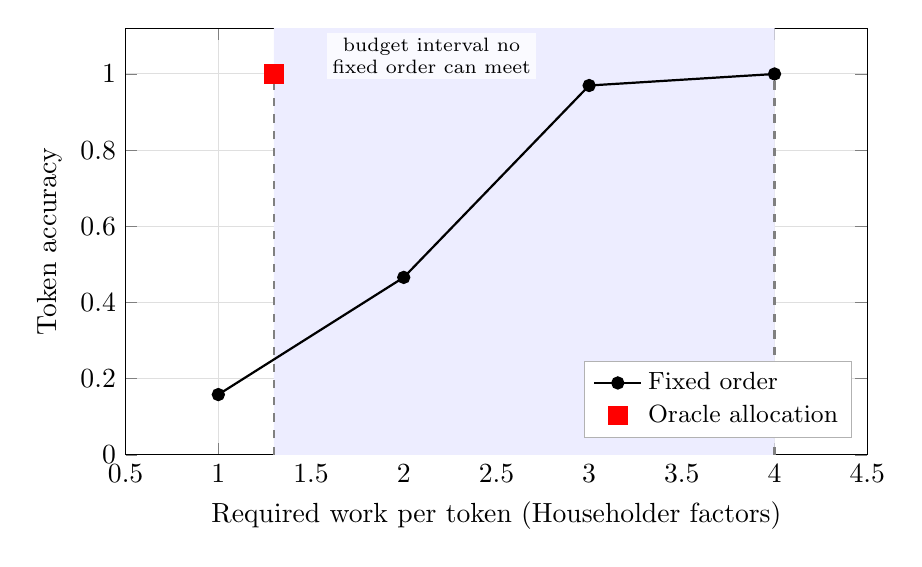
\begin{tikzpicture}
	\begin{axis}[
		width=11cm, height=7cm,
		xlabel={Required work per token (Householder factors)},
		ylabel={Token accuracy},
		xmin=0.5, xmax=4.5, ymin=0, ymax=1.12,
		grid=major, grid style={gray!25},
		legend style={at={(0.98,0.04)}, anchor=south east, draw=gray!60, fill=white, font=\small},
		legend cell align={left},
		every axis plot/.append style={thick},
	]
	\addplot[draw=none, fill=blue!7, forget plot] coordinates {
		(1.300,0) (4.0,0) (4.0,1.12) (1.300,1.12)
	} \closedcycle;
	\node[font=\scriptsize, align=center, anchor=north, fill=white, fill opacity=0.75,
	      text opacity=1, inner sep=2pt] at (axis cs:2.15,1.11)
		{budget interval no\\ fixed order can meet};
	\addplot[mark=*, color=black] coordinates {
		(1.0,0.1583) (2.0,0.4659) (3.0,0.9696) (4.0,0.9999)
	};
	\addlegendentry{Fixed order}
	\addplot[only marks, mark=square*, mark size=3.2pt, color=red] coordinates {
		(1.300,0.9999)
	};
	\addlegendentry{Oracle allocation}
	\addplot[dashed, color=gray, forget plot] coordinates {(1.300,0) (1.300,0.9999)};
	\addplot[dashed, color=gray, forget plot] coordinates {(4.0,0) (4.0,0.9999)};
	\end{axis}
	\end{tikzpicture}
	\caption{Accuracy against required work at $p = 0.10$. The oracle allocation attains the accuracy of the $n_h = 4$ model at $1.300$ factors per token. No fixed order occupies the interval between these two points, because the fixed order is integer-valued.}
	\label{fig:matched}
\end{figure}

Table \ref{table:sweep} extends the comparison across three mixture rates. In
each case the oracle allocation matches the accuracy of the cheapest fixed order
that solves the task, at a fraction of the required work.

\begin{table}[ht]
	\caption{Oracle allocation against the cheapest adequate fixed order}
	\centering
	\begin{tabular}{c c c c c}
		\hline\hline
		$p$ & $E[D]$ & Fixed $n_h{=}4$ & Oracle allocation & Reduction \\ [0.5ex]
		\hline
		0.05 & 1.150 & 0.9999 at cost 4 & 1.0000 at cost 1.150 & $3.48\times$ \\
		0.10 & 1.300 & 0.9999 at cost 4 & 0.9999 at cost 1.300 & $3.08\times$ \\
		0.25 & 1.752 & 0.9997 at cost 4 & 0.9999 at cost 1.752 & $2.29\times$ \\ [1ex]
		\hline
	\end{tabular}
	\label{table:sweep}
\end{table}

Because a fixed order is integer-valued, it occupies only the discrete points
$1, 2, 3, 4$ on the cost axis. For any computational budget $B$ satisfying
$E[D] \le B < D_{\max}$, no fixed-order model both meets the budget and solves
the task, whereas an adaptive model does. The width of that interval narrows as
$p$ increases, in agreement with $E[D] = 1 + 3p$.

Two properties of these figures govern their interpretation. The oracle condition
is a control in which the correct per-token order is supplied from ground truth;
it establishes the reduction attainable by a correct allocation and is
independent of whether a gate can learn that allocation. The reduction is in
required work per token and not in elapsed time: under the dense execution
strategy of Section 3.5 the adaptive condition ran in $756$\,s against $761$\,s
for the full-cost condition, a difference within measurement noise, because
disabled factors are still materialised and multiplied by zero.

\section{Training Stability and Its Consequences for Measurement}

Fifty training runs of the unmodified architecture were conducted across four
alphabets at $20{,}000$ steps with a constant learning rate, with the data held
fixed and only the run varied. Table \ref{table:census} reports the outcome.

\begin{table}[ht]
	\caption{Escape fraction over repeated runs of identical configurations}
	\centering
	\begin{tabular}{P{4.0cm} c c P{3.0cm}}
		\hline\hline
		Configuration & Escapes / runs & Rate & Outcome distribution \\ [0.5ex]
		\hline
		$A_5$ five-cycles, $n_h{=}2$ & 4 / 14 & 0.29 & bimodal \\
		$A_5$ with double transp., $n_h{=}2$ & 2 / 10 & 0.20 & bimodal \\
		$A_5$ with double transp., $n_h{=}4$ & 1 / 10 & 0.10 & bimodal \\
		$S_5$ with transposition, $n_h{=}4$ & 3 / 10 & 0.30 & bimodal \\ [1ex]
		\hline
	\end{tabular}
	\label{table:census}
\end{table}

Outcomes on these configurations are bimodal. A run either escapes the loss
plateau and reaches approximately $0.99$ token accuracy, or remains at chance
accuracy near $0.04$; intermediate outcomes are rare. Escape is abrupt, with the
loss falling by two orders of magnitude within a single logging interval, and
occurs anywhere between step $5{,}000$ and step $20{,}000$. Non-determinism in the
bfloat16 kernels alone is sufficient to select between the two outcomes: an
identical configuration under an identical seed has produced both.

Two consequences follow. The first is methodological: a single run of such a
configuration carries no information about the configuration, and the appropriate
summary statistic is the escape fraction over repeated runs. Distinguishing an
escape rate of $0.25$ from one of $0.75$ at the $5\%$ level with $80\%$ power
requires approximately $20$ runs per condition, which is the budget adopted for
subsequent experiments on these configurations. Under the measured rates, the
best run obtained on the $S_5$ alphabet reaches token accuracy $0.9994$ and
sequence accuracy $0.9415$, with accuracy $0.9995$ on even targets and $0.9994$
on odd, establishing that the configuration is solvable and that the difficulty
is one of optimisation rather than expressivity.

The second consequence concerns the scope of the proposed mechanism. Table
\ref{table:benefit} sets the measured escape rates against the reduction that a
correct allocation would deliver on each configuration.

\begin{table}[ht]
	\caption{Available reduction against training reliability}
	\centering
	\begin{tabular}{P{3.6cm} P{4.2cm} P{3.0cm}}
		\hline\hline
		Available reduction & Configurations & Trains reliably \\ [0.5ex]
		\hline
		$2.29\times$ -- $3.48\times$ & $p = 0.05,\ 0.10,\ 0.25$ & yes, $\ge 0.9997$ \\
		$1.28\times$ & $S_5$ with transposition & 3 / 10 \\
		$1.00\times$ & $A_5$ alphabets & 1--4 / 10 \\ [1ex]
		\hline
	\end{tabular}
	\label{table:benefit}
\end{table}

Every configuration that trains reliably is one in which adaptive allocation
reduces required work by a factor between $2.3$ and $3.5$. Every configuration
that trains unreliably is one in which the available reduction is $1.28\times$ or
less, and for the $A_5$ alphabets it is exactly unity, since the requirement is
constant across the alphabet and no allocation can improve on a fixed order. The
region in which the architecture is least stable and the region in which the
proposed mechanism is useful are therefore disjoint.

\section{Error Characterisation}

The structure of the errors made by under-provisioned models was examined at
$p = 0.10$. Table \ref{table:forensics} reports the results.

\begin{table}[ht]
	\caption{Error structure at $p = 0.10$}
	\centering
	\begin{tabular}{P{4.6cm} c c c}
		\hline\hline
		& $n_h{=}1$ & $n_h{=}3$ & $n_h{=}4$ \\ [0.5ex]
		\hline
		Token / sequence accuracy & 0.1822 / 0.0000 & 0.9740 / 0.7145 & 0.9999 / 0.9940 \\
		Per-high-requirement-token success & 0.7124 & 0.9947 & 1.0000 \\
		Mean error-run length & 30.13 & 2.00 & 1.11 \\
		Sequences containing any error & 2000 / 2000 & 571 / 2000 & 12 / 2000 \\ [1ex]
		\hline
	\end{tabular}
	\label{table:forensics}
\end{table}

Errors are clustered rather than independent, and they are not absorbing. Two
models of the error process were stated in advance and are both inconsistent with
the measurements: independent per-position errors predict a sequence accuracy of
$0.974^{128} = 0.034$ for the $n_h = 3$ model against $0.7145$ observed, while
permanent corruption of the state predicts a token accuracy of $0.746$ against
$0.9740$ observed. The $n_h = 3$ model recovers from errors, with a median
error-run length of a single position. Since a corrupted group-tracking state
possesses no mechanism by which to correct itself, information sufficient for
recovery is being carried outside the transition matrices, and the additive
channel of the recurrence is the natural candidate.

\section{End-to-End Training of the Halting Gate}

The learned condition was evaluated at $p = 0.10$ against the fixed-order and
oracle conditions, at four budget weights $\gamma \in \{0,\ 0.01,\ 0.03,\ 0.1\}$
and three random seeds, giving $18$ training runs conducted within a single
invocation. The budget penalty was held at zero for $4{,}000$ steps and then
increased linearly over a further $4{,}000$. Gates were evaluated in hard mode,
so every reported cost is an integer factor count.

In one of the three seeds the gate converged to the oracle allocation. Table
\ref{table:gate} reports that seed.

\begin{table}[ht]
	\caption{Learned allocation against the oracle, for the seed in which the gate converged}
	\centering
	\begin{tabular}{P{3.4cm} c c c c c}
		\hline\hline
		Condition & Token & Sequence & Cost & Mean abs.\ error & Correlation \\ [0.5ex]
		\hline
		Fixed, $n_h = 4$ & 0.9998 & 0.9885 & 4.000 & --- & --- \\
		Oracle allocation & 0.9996 & 0.9770 & 1.298 & 0.00 & 1.00 \\
		Learned, $\gamma = 0.03$ & 0.9999 & 0.9910 & \textbf{1.298} & \textbf{0.00} & \textbf{1.00} \\
		Learned, $\gamma = 0.1$ & 1.0000 & 0.9970 & \textbf{1.298} & \textbf{0.00} & \textbf{1.00} \\ [1ex]
		\hline
	\end{tabular}
	\label{table:gate}
\end{table}

The mean absolute allocation error of zero is taken over $256{,}000$ evaluated
tokens. The decisive measurement is the allocation grouped by requirement, shown
in Figure \ref{fig:alloc}, since a gate that reached the correct average by
closing uniformly across all tokens would produce the same mean cost while
carrying no information. Every token of requirement one received exactly one
factor and every token of requirement four received exactly four, matching the
oracle in both groups. Two independent budget weights produced the same
allocation. The differences in accuracy relative to the oracle lie within the
noise floor established in Section 3.7.

\begin{figure}[ht]
	\centering
	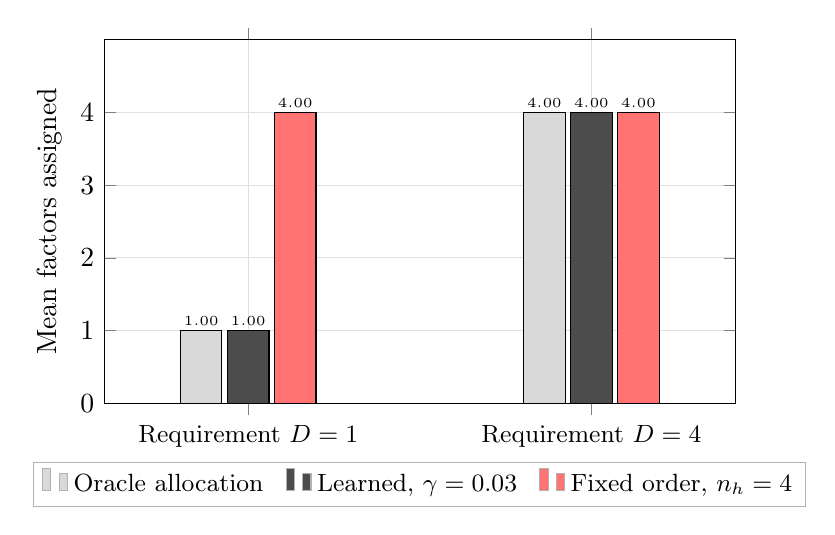
\begin{tikzpicture}
	\begin{axis}[
		width=9.6cm, height=6.2cm,
		ybar,
		bar width=15pt,
		symbolic x coords={D1, D4},
		enlarge x limits=0.42,
		xtick=data,
		xticklabels={Requirement $D=1$, Requirement $D=4$},
		xticklabel style={font=\small},
		ymin=0, ymax=5.0,
		ytick={0,1,2,3,4},
		ylabel={Mean factors assigned},
		legend style={at={(0.5,-0.16)}, anchor=north, legend columns=3,
		              draw=gray!60, font=\small, /tikz/every even column/.append style={column sep=6pt}},
		legend cell align={left},
		grid=major, grid style={gray!25},
		nodes near coords={\pgfmathprintnumber[fixed, zerofill, precision=2]{\pgfplotspointmeta}},
		nodes near coords style={font=\tiny, inner sep=1.5pt},
	]
	\addplot[fill=gray!30] coordinates {(D1, 1.00) (D4, 4.00)};
	\addlegendentry{Oracle allocation}
	\addplot[fill=black!70] coordinates {(D1, 1.00) (D4, 4.00)};
	\addlegendentry{Learned, $\gamma = 0.03$}
	\addplot[fill=red!55] coordinates {(D1, 4.00) (D4, 4.00)};
	\addlegendentry{Fixed order, $n_h = 4$}
	\end{axis}
	\end{tikzpicture}
	\caption{Mean number of factors assigned, grouped by the token's requirement, over $230{,}531$ tokens of requirement one and $25{,}469$ of requirement four. The learned allocation is indistinguishable from the oracle in both groups, while the fixed-order model spends four factors on every token regardless of requirement.}
	\label{fig:alloc}
\end{figure}

In the remaining two seeds the gate did not depart from full order, holding cost
at exactly $4.000$ at every budget weight including the largest, with correlation
$0.00$ against the requirement. Across the three seeds the gate therefore
converged to the oracle allocation in one, and this is reported as a fraction in
accordance with the protocol of Section 3.7 rather than as a mean over seeds.

Two further observations bear on this outcome. First, task accuracy lies between
$0.98$ and $1.00$ in all eighteen runs, including those in which the gate did not
close; the variability is confined to the allocation and is independent of the
accuracy bimodality characterised in Section 4.6. Second, in the $\gamma = 0$
control, in which the gate is present but never penalised, the converging seed
still reached cost $3.369$ with correlation $0.43$, assigning a mean of $3.30$
factors to requirement-one tokens against $4.00$ to requirement-four tokens,
while the remaining seeds held at $4.000$. The task loss alone therefore exerts
pressure towards closure on low-requirement tokens, and the difference between
seeds is established before the budget penalty takes effect.

\section{Discussion}

The results divide into three groups, and the distinctions between them are
material to their interpretation.

The reachability bounds and the order-requirement model are established by
explicit construction in double-precision arithmetic, with no optimiser involved,
and hold independently of any training outcome. The closure experiment provides
the corresponding empirical confirmation, separating perfectly along the
predicted variable while excluding alphabet size as an alternative explanation.

The matched-computation results establish what a correct per-token allocation
achieves: accuracy equal to the cheapest adequate fixed order at $2.29$ to $3.48$
times less required work, across three mixture rates. Because the allocation in
this condition is supplied from ground truth, these figures bound the attainable
reduction rather than demonstrate that it is attainable by a learned mechanism.

The end-to-end results address that remaining question directly. A gate trained
under a penalty on expected computation, receiving no supervision on the
allocation, reproduced the oracle allocation exactly in one of three seeds,
assigning the correct integer factor count to every one of $256{,}000$ evaluated
tokens. The allocation was recovered rather than approximated, and it was
recovered at two independent budget weights. Establishing the conditions under
which this outcome occurs reliably is the principal objective of the continuing
work described in Chapter 5.

A final observation concerns the interaction between Sections 4.5 and 4.6. The
configurations on which the architecture trains least reliably are precisely
those on which adaptive allocation offers a reduction of $1.28\times$ or less,
while every configuration offering a reduction above $2.29\times$ trains to
$0.9997$ or better. The instability of the base architecture and the operating
region of the proposed mechanism therefore do not overlap, which bounds the
extent to which the former limits the latter.
\null
